\documentclass{beamer}
\usepackage[utf8]{inputenc}
\usepackage{graphicx}
\usetheme{Madrid}

%Information to be included in the title page:
\title{FaaS}
\author{Eirik, Orestis, Rurik}
\institute{Unit}
\date{2019}

\begin{document}
\frame{\titlepage}

\begin{frame}
\frametitle{What will we talk about?}
\begin{itemize}
  \item What do me mean by FaaS?
  \item Benefits of FaaS
  \item Challenges of FaaS
  \item Understanding cost and cost implications
  \item Concrete examples
  \begin{itemize}
    \item REST API
    \item CD-platform
  \end{itemize}
  \item Summary
\end{itemize}
\end{frame}

\begin{frame}
\frametitle{What do we mean by FaaS?}
Simply put: AWS Lambda and managed services like DynamoDB
\end{frame}

\begin{frame}
\frametitle{Benefits of FaaS}
\begin{itemize}
  \item Lower costs
  \item Simplicity
  \item More testable architecture
  \item Replicability
  \item ``Driftløshet''
\end{itemize}
\end{frame}

\begin{frame}
\frametitle{Challenges of FaaS I}
Challenges:
\begin{itemize}
  \item Vendor lock-in
  \item New idiom, a lot to learn
  \item Not suited to every task
  \item Accidental costs can accumulate
  \item Possible to make a real mess
\end{itemize}
\end{frame}

\begin{frame}
\frametitle{Challenges of FaaS II}
How to deal with them:
\begin{itemize}
  \item Portable code 
  \begin{itemize}
	\item   but don't strive for project-defeating generics
  \end{itemize}  
  \item Understand the offerings, learn about Infrastructure As Code (IAC)
  \item Many things can be solved with Lambdas. (But should they?) 
  \item Keep an eye on what costs are accumulating by setting up cost reports, automate resource deprovisioning
  \item Discipline is important: 
  \begin{itemize}
    \item TDD \& BDD/FDD are essential
    \item Code hygiene and QA equally so
    \item having continuous deployment as a constant and understood aim
    \item IAC is an absolute
  \end{itemize}
\end{itemize}
\end{frame}

\begin{frame}
\frametitle{Understanding costs \& cost implications}
Cheap:
\begin{itemize}
  \item Some stuff costs a lot
  \item Some stuff costs little, if it is used correctly
\end{itemize}
Cheap isn't always good
\begin{itemize}
  \item Some stuff is cheaper to implement in different ways
  \begin{itemize}
    \item Cost for light usage for some services is high (CloudSearch)
  \end{itemize}
  \item Some stuff is more performant if implemented in different ways
  \begin{itemize}
    \item Long-running and/or processor-intensive processes are better run in EC2 as Lambda becomes expensive in these cases
  \end{itemize}
\end{itemize}
Basically, know your needs; know the platform; use the appropriate technology.

\end{frame}

\begin{frame}
\frametitle{Concrete example: REST API (A Serverless Server)}
\begin{itemize}
\item A Jersey server as a function.
\item Advantages
\begin{itemize}
\item The server starts with very small delay (milliseconds)
\item Server dies after few minutes without requests
\item Cost for low/moderate traffic: low
\item Scales automatically
\item No maintenance
\item The Jersey server can be ported into an EC2 instance with very few code modifications
\item Extremely easy to replicate the production environment
\end{itemize}
\item Disadvantages
\begin{itemize}
\item Cost for high traffic: unknown 
\item Can have problems with timeouts for very heavy queries. 
\end{itemize}

\end{itemize}
\end{frame}

\begin{frame}
\frametitle{Concrete example: REST API}
\begin{figure}
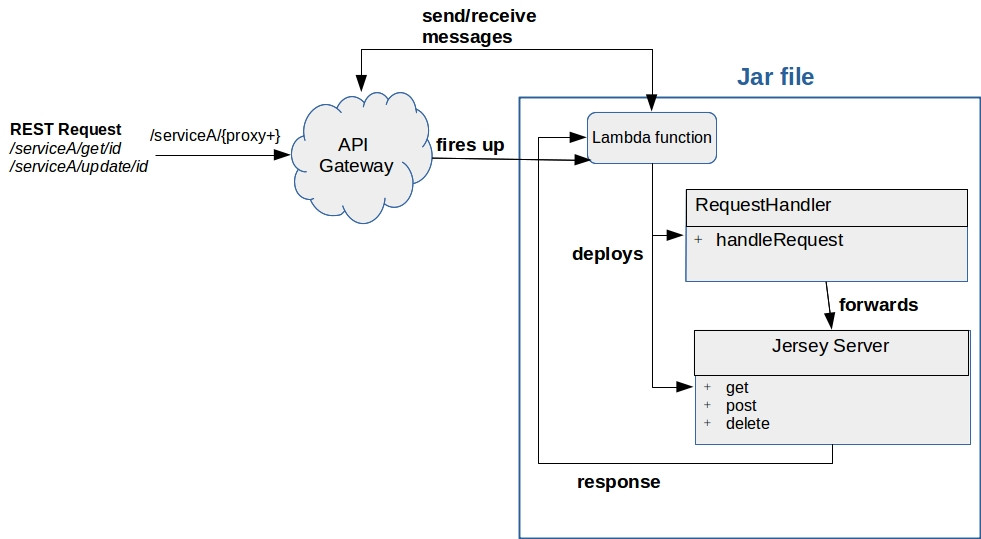
\includegraphics[scale=0.3]{rest.jpeg}
\end{figure}

\end{frame}

\begin{frame}
\frametitle{Concrete example: CD-platform}
\begin{figure}
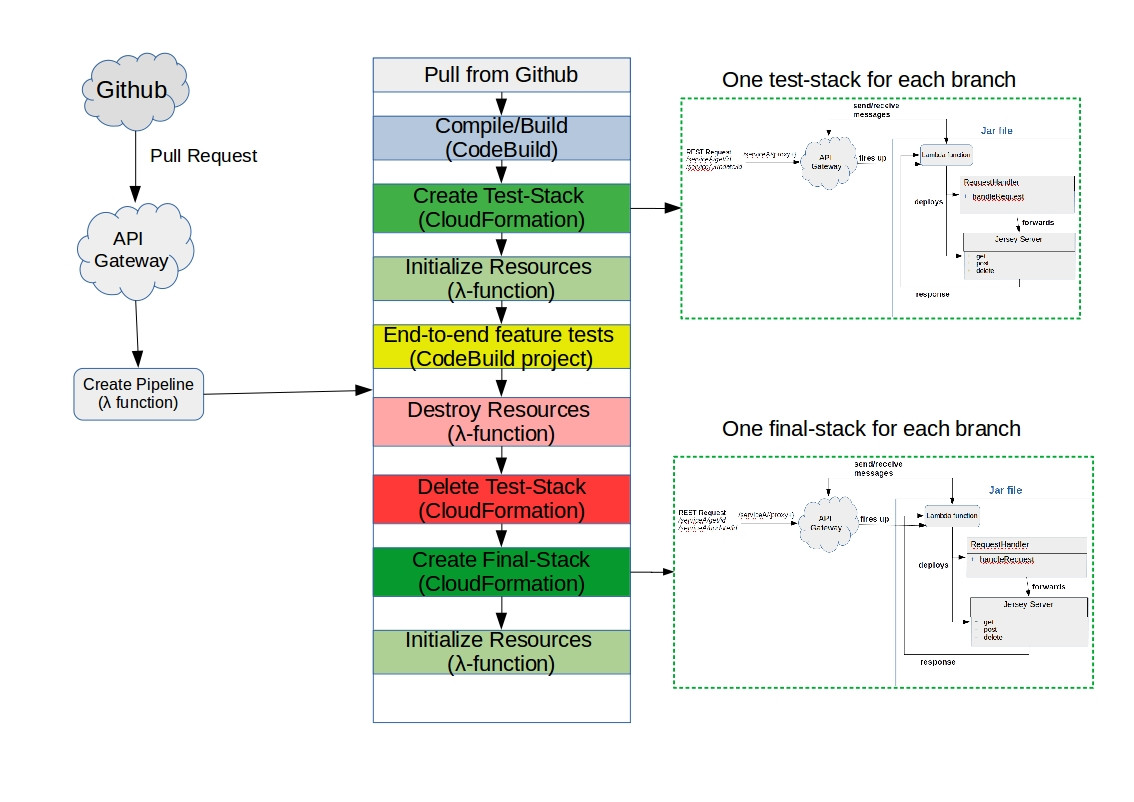
\includegraphics[scale=0.3]{cd.jpeg}
\end{figure}
\end{frame}

\begin{frame}

\frametitle{Summary}
\begin{itemize}
  \item Infrastructure as code is alpha \& omega
  \item Automated deployment of services ("Driftløs")
  \item Choose the right DevOps approach and develop it
  \begin{itemize}
    \item Test-first, test-last and test everything inbetween
    \item CD
    \item Stamp out laziness
  \end{itemize}
  \item Read the DORA report for inspiration
\end{itemize}
\end{frame}
\end{document}
